\subsection{Macaque motor cortex spike data in an active reaching task}
\label{subsection:churchland_results}

% Given the outline we discussed before:
% 1. Introduce the dataset and discovery workflow.
% 2. Show 2–4 interpretable features discovered with NLDisco.
% 3. Explain plots and metrics.
% 4. Briefly introduce CEBRA and LangevinFlow.
% 5. Compare recovery of the identified features and metrics across all methods, incl. decoding performance.

To test NLDisco on real neural data with unknown ground-truth representations, and to compare to other established neural LVM models, we analyze neural and behavioral data from a popular macaque motor control task~\citep{churchland_2012_population_dynamics}, prepared by Brainsets~\citep{azabou_2023_unified}. Briefly, the task requires the macaque to wait for a go cue before reaching to a visual target with a hand-controlled cursor while avoiding virtual barriers in different configurations (\autoref{figure:task_overview}b).

We analyze one experiment comprising 1,906 retained trials across 27 configurations with nine total target locations. Unsorted spikes were recorded from dorsal premotor and primary motor cortex using $N=191$ Utah array channels, and neural and behavioral data are binned at 50 ms. To try to find both instantaneous and temporally-evolving features, we use $S=10$ to capture 500 ms of activity per example, and train a two-level Matryoshka TW-SED with $(D_1,k_1)=(96,8)$, $(D_2,k_2)=(192,16)$, and $B=1024$. Inspection of latent-conditioned kinematics and task conditions guides feature visualization: behavioral descriptions are developed from trained latents, then fixed for comparison.

Among many features found (see \hyperref[subsubsection:churchland_results_additional]{\ref*{subsubsection:churchland_results_additional}}), here we highlight two that together span kinematics and task conditions: 1) \textit{recent deceleration}: a speed slope $\leq-75$ mm/s$^2$ over the preceding 250 ms; 2) \textit{fast leftward target reach}: a movement within $45^\circ$ of leftward at endpoint speed $\geq500$ mm/s on trials with target positioned at $(-144,-52)$ mm of screen center. We visualize them by plotting the probability of latent activation conditioned on behavioral and environmental variables (\autoref{fig:churchland_results}a), and quantify these associations using standard metrics for coverage (\metric{Cov}), specificity (\metric{Spec}), selectivity (\metric{Sel}), and discriminability (\metric{AUROC}; \autoref{fig:churchland_results}b,c). \metric{Cov} measures how often a latent activates within the condition, \metric{Spec} how often it remains inactive outside it, \metric{Sel} summarizes this preference, and \metric{AUROC} measures discrimination across activation thresholds (definitions in \hyperref[subsubsection:latents_evaluation_details]{\ref*{subsubsection:latents_evaluation_details}}). All metrics range from 0 to 1, with a higher value indicating a better score.

% We then quantify their selectivity and discriminability with two standard metrics: 1) the selectivity of latent activation for the feature-defining condition ($\metric{Sel}$); 2) the area under the receiver operating characteristic curve ($\metric{AUROC}$), which measures how well latent activity discriminates between windows satisfying the defining condition and those that do not (\autoref{fig:churchland_results}b; see \hyperref[subsubsection:latents_evaluation_details]{\ref*{subsubsection:latents_evaluation_details}} for mathematical definitions).

\begin{figure}[tb]
    \centering
    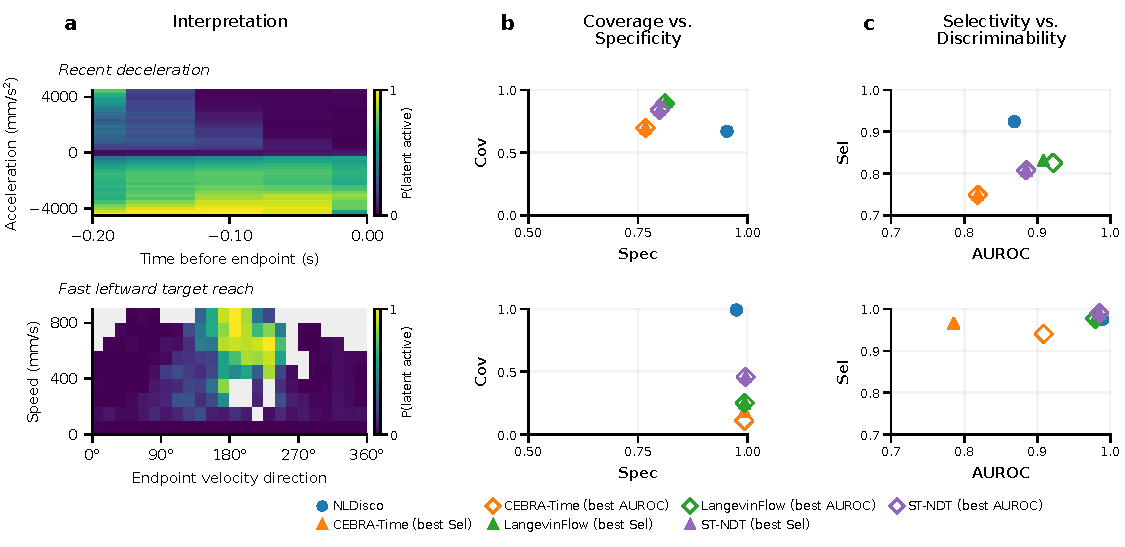
\includegraphics[width=\linewidth]{figures/rebuttal/change01_stndt/figure4.pdf}
    \caption{\textbf{Interpreting and comparing features in 192-dimensional representations.} (\textbf{a}) NLDisco latent activation probability conditioned on speed slope over the preceding 250 ms (top, latent 83) or endpoint velocity direction and speed (bottom, latent 20), for the second level ($D=192$, $k=16$) of the two-level Matryoshka TW-SED trained on examples of $S=10$ with 50 ms bins. Both heatmaps pool data from all valid experiment trials; they do \textit{not} restrict observations to the scored conditions (gray cells have fewer than 10 distinct trials). (\textbf{b}) \metric{Cov} versus \metric{Spec} and (\textbf{c}) \metric{Sel} versus \metric{AUROC} for the same NLDisco latents and the CEBRA-Time, LangevinFlow, and ST-NDT (191-dimensional) latents that best match these features. Source activity traceback appears in \autoref{figure:churchland_traceback}.}
    \label{fig:churchland_results}

\end{figure}

We then compare results to other popular neural LVMs. For fair comparisons focused on the main goal of unsupervised interpretable latent discovery, we consider published methods (\autoref{table:method_comparisons}) that: 1) prioritize an interpretable latent space; 2) do not require multimodal or trial-structured data. Here we show results from CEBRA-Time, the label-free variant of CEBRA (which contrastively learns a continuous neural embedding space~\citep{schneider_2023_cebra}), LangevinFlow (which models neural activity through structured, stochastic dynamics~\citep{song_2025_langevinflow} and is a top-performing sequential variational method on Neural Latents Benchmark (NLB)~\citep{pei_2022_nlb}), and ST-NDT~\citep{le_2022_stndt} (a spatiotemporal Transformer trained with masked spike prediction and a contrastive loss, and another top-ranked entry on NLB).

We set the latent space to 192 dimensions for CEBRA-Time and LangevinFlow to match the SED's, while ST-NDT's width is set to 191 as it is tied to the 191 input channels. We perform 12-run sweeps for each method, varying temperature and positive-pair lag for CEBRA-Time, learning rate and regularization-ramp duration for LangevinFlow, and contrastive-loss weight, learning rate, and dropout for ST-NDT (see \hyperref[subsubsection:churchland_results_additional]{\ref*{subsubsection:churchland_results_additional}} for full sweep configurations). For each baseline method, we select the model with the highest mean \metric{AUROC} across features using their best matching latents. And to give the baselines a better opportunity to demonstrate both selectivity and discrimination, we report up to two latents per feature -- the highest-\metric{Sel} and highest-\metric{AUROC} dimensions -- alongside the illustrative NLDisco latent. As in \hyperref[subsection:synthetic_results]{\ref*{subsection:synthetic_results}}, this is a targeted search for known features, not a comparison of what each method would discover without specified behavioral descriptions.

As expected, all three baselines recover these features. For \textit{recent deceleration}, NLDisco has the highest $\metric{Spec}$ and $\metric{Sel}$, but lower $\metric{Cov}$ than the baselines, while LangevinFlow has the highest $\metric{AUROC}$ and ST-NDT falls between CEBRA-Time and LangevinFlow on all four metrics. For \textit{fast leftward target reach}, NLDisco covers nearly all condition-positive examples with much higher $\metric{Cov}$ than the baselines. All shown latents are highly selective for this feature, with NLDisco, LangevinFlow, and ST-NDT latents also highly discriminative; ST-NDT's latent has the highest $\metric{Spec}$ and $\metric{Sel}$ of all methods, at less than half of NLDisco's $\metric{Cov}$. At equal $\metric{Cov}$, the NLDisco latents have the highest $\metric{Sel}$ for every feature across baseline activation thresholds (\hyperref[subsubsection:rebuttal_threshold_sensitivity]{\ref*{subsubsection:rebuttal_threshold_sensitivity}}). These comparisons highlight why the metrics should be considered together: a highly selective latent need not detect most condition-positive examples or discriminate well across activation thresholds, as ROC curves further illustrate (\autoref{figure:churchland_rocs}).

Last, we assess feature decoding from each displayed latent and the full latent space using identical $\ell_2$-regularized logistic regression. We report test balanced accuracy with validation-selected regularization and decision thresholds, using a 0.8/0.1/0.1 whole-trial split (\autoref{table:churchland_comparison}; shared protocol in \hyperref[paragraph:latent_decoding]{\ref*{subsubsection:latents_evaluation_details}}). We see all methods perform well on feature decoding from the full latent space, while single-latent decoding favors NLDisco, LangevinFlow, and ST-NDT. With a shared Poisson readout, ST-NDT's representation reconstructs held-out spike counts best, and NLDisco's reconstructs them as well as LangevinFlow's and better than CEBRA-Time's. Among the models' own decoders, NLDisco's reconstructs best (\autoref{table:rebuttal_reconstruction}). Overall, we find that CEBRA, LangevinFlow, and ST-NDT can contain recoverable behavioral information, but their objectives do not explicitly favor individual feature detectors. NLDisco, meanwhile, makes these a natural starting point for discovery: inspect activating examples, formulate behavioral interpretations, and quantify selectivity and discrimination. Here, NLDisco supports this direct, latent-centered workflow while retaining strong decoding performance. We compare end-to-end feature discovery of these methods in \hyperref[subsection:aeon_results]{\ref*{subsection:aeon_results}} and \hyperref[subsubsection:rebuttal_discovery_comparison]{\ref*{subsubsection:rebuttal_discovery_comparison}}, and we compare training times in \autoref{figure:training_time_h100}.

\begin{table}[tb]
    \centering
    {\setlength{\tabcolsep}{3pt}\resizebox{\linewidth}{!}{\begin{tabular}{l*{12}{r}}
\toprule
 & \multicolumn{6}{c}{\textit{Recent deceleration}} & \multicolumn{6}{c}{\textit{Fast leftward target reach}} \\
\cmidrule(lr){2-7}\cmidrule(lr){8-13}
Method & \metric{Cov} & \metric{Spec} & \metric{Sel} & \metric{AUROC} & \shortstack{Single\\Decode} & \shortstack{All\\Decode} & \metric{Cov} & \metric{Spec} & \metric{Sel} & \metric{AUROC} & \shortstack{Single\\Decode} & \shortstack{All\\Decode} \\
\midrule
NLDisco & 0.671 & \textbf{0.953} & \textbf{0.924} & 0.868 & 0.768 & \textbf{0.918} & \textbf{0.991} & 0.975 & 0.975 & \textbf{0.989} & \textbf{0.981} & \textbf{0.995} \\
CEBRA-Time (best \metric{Sel}) & 0.698 & 0.767 & 0.749 & 0.818 & 0.729 & 0.899 & 0.183 & 0.993 & 0.965 & 0.785 & 0.718 & 0.989 \\
CEBRA-Time (best \metric{AUROC}) & 0.698 & 0.767 & 0.749 & 0.818 & 0.729 & 0.899 & 0.112 & 0.993 & 0.940 & 0.908 & 0.827 & 0.989 \\
LangevinFlow (best \metric{Sel}) & \textbf{0.909} & 0.816 & 0.831 & 0.908 & \textbf{0.862} & 0.902 & 0.252 & 0.994 & 0.975 & 0.979 & 0.915 & 0.958 \\
LangevinFlow (best \metric{AUROC}) & 0.892 & 0.812 & 0.825 & \textbf{0.921} & 0.850 & 0.902 & 0.252 & 0.994 & 0.975 & 0.979 & 0.915 & 0.958 \\
ST-NDT (best \metric{Sel}) & 0.841 & 0.800 & 0.808 & 0.885 & 0.818 & 0.911 & 0.460 & \textbf{0.996} & \textbf{0.990} & 0.985 & 0.932 & 0.991 \\
ST-NDT (best \metric{AUROC}) & 0.841 & 0.800 & 0.808 & 0.885 & 0.818 & 0.911 & 0.460 & \textbf{0.996} & \textbf{0.990} & 0.985 & 0.932 & 0.991 \\
\bottomrule
\end{tabular}
}}
    \caption{\textbf{Feature recovery and decoding.} \metric{Cov}, \metric{Spec}, \metric{Sel}, \metric{AUROC} and feature decoding scores for features and latents shown in \autoref{fig:churchland_results}. ``Single decode'' uses individual latents, while ``All decode'' uses the entire latent space. \metric{Decode} reports test balanced accuracy from logistic regression with validation-selected decision thresholds and a 0.8/0.1/0.1 whole-trial split (\hyperref[paragraph:latent_decoding]{\ref*{subsubsection:latents_evaluation_details}}). Column maxima are bolded, including ties.}
    \label{table:churchland_comparison}
\end{table}
